\documentclass[12pt,a4paper,notitlepage]{report}
\usepackage{fullpage}
\usepackage{lastpage}
\usepackage{graphicx}
\usepackage[overlay]{textpos}
\usepackage{fancyhdr}
\usepackage{extramarks}
\usepackage{xfrac}
\usepackage{textcomp}
\usepackage[hidelinks,colorlinks,urlcolor=blue]{hyperref}

%% Use fancyhdr to get our desired headers and footers
\pagestyle{fancy}
\renewcommand{\headrulewidth}{0pt}% removes header line
\fancypagestyle{plain}{% for chapter starting pages
  \fancyhf{}% clears header fields
  \rfoot{\hyperlink{contents}{Return to contents}}}

%% Setup footer for all other pages
\fancyhf{}%clear all fields
\rfoot{\hyperlink{contents}{Return to contents}}% links the TOC at the center of the page footer
\cfoot{\thepage\ of \pageref*{LastPage}}
\lfoot{\leftmark}
\renewcommand{\chaptermark}[1]{%
  \markboth{#1}{}}

%%TOC Hyperlink Setup


%%Document start
\begin{document}

%% Macros Section
\newcommand{\newrecipe}[2] {%parameter1 is the recipe name parameter 2 is the hyperlink to original content (if applicable).
	\newpage
	\phantomsection
	\addcontentsline{toc}{section}{#1}
	\section*{
	\center {\Huge \href{#2}{#1}}
%	\centerline {\Huge \href{#2}{#1}}
	}
}

%%List Style Setup
\newenvironment{ingredients-list}{
  \begin{itemize}
  \setlength{\itemsep}{1pt}
  \setlength{\parskip}{0pt}
  \setlength{\parsep}{0pt}
}{
  \end{itemize}
}


%%Title Page
\title{Tried and Tested}
\date{}
\author{}
\maketitle
\begin{figure}[h!]
\centering

\includegraphics[scale=1]{./img/recipe-book.jpg}
\end{figure}
\thispagestyle{empty}
\newpage

%%TOC page(s)
\hypertarget{contents}{}%Navigation target to return to Toc from any page
\hypersetup{
  colorlinks,
  linkcolor=blue,
  linktoc=all
}
\tableofcontents

%%Chapter - Split into separate file if too large
\chapter{Finger Food}
%%Start recipe
\newrecipe{Caramelised Onion Tarts}{}
\section*{Directions}
\begin{enumerate}
	\item Make the balsamic onion jam as directed in the \hyperlink{caramelised_onion}{recipe} on page \pageref{caramelised_onion}
	\item Spoon mixture into pre-made pastry cases and top with crumbled feta, goats cheese or blue cheese.
\end{enumerate}
%%End recipe

%%Start recipe
\newrecipe{Roast Beef Canapes}{http://www.taste.com.au/recipes/18552/roast_beef_canapes}
\section*{Ingredients}
\begin{ingredients-list}
	\item 30cm-long baguette bread
	\item olive oil cooking spray
	\item 200g sliced rare roast beef, cut into strips
	\item 200g roasted red capsicum, thinly sliced
	\item Horseradish mayonnaise
	\item \sfrac{1}{2} cup whole-egg mayonnaise
	\item 1 tablespoon horseradish cream
	\item 1\sfrac{1}{2} teaspoons Dijon mustard 
\end{ingredients-list}
\section*{Directions}
\begin{enumerate}
	\item Preheat oven to 180°C. Trim ends from bread. Cut into 24, 5mm-thick slices. Place bread slices, in a single layer, on 2 oven trays. 
	Spray with oil. Bake for 8 to 10 minutes, swapping trays over halfway through cooking, or until light golden. Remove to a wire rack to cool completely.
	\item Make horseradish mayonnaise: Combine mayonnaise, horseradish cream and mustard in a small bowl. Season with salt and pepper.
	\item Top each bread slice with roast beef. Dollop with horseradish mayonnaise and top with capsicum. Season with pepper. Serve immediately.
\end{enumerate}
%%End recipe

%%Start recipe
\newrecipe{Corn Fritters}{}
\section*{Ingredients}
\begin{ingredients-list}
	\item 420g can corn kernels, drained
	\item 1 cup or 150g self-raising flour
	\item 2 shallots, trimmed and sliced
	\item 2 eggs
	\item \sfrac{1}{4} cup or 60ml milk
	\item Butter, to grease
\end{ingredients-list}
\section*{Directions}
\begin{enumerate}
	\item To make the fritters, combine corn kernels, flour and shallot in a bowl. Make a well in the centre and add the eggs and milk.
		Stir gradually incorporating liquid with dry ingredients until combined.
	\item Lightly grease a frying pan with butter. Heat over a medium-low heat. Cook 2 corn fritters at a time - l/4 cup corn mixture makes 1 fritter.
		Cook for 2-3 minutes each side, or until golden.
	\item Set aside. Repeat with remaining mixture
\end{enumerate}
%%End recipe

%%Start recipe
\newrecipe{Chicken Satays}{http://www.taste.com.au/recipes/5925/chicken_satays}
\section*{Ingredients}
\begin{ingredients-list}
	\item 1 cup coconut cream
	\item 2 tbsp. good-quality mild curry powder
	\item 4 garlic cloves
	\item 2 tbsp. brown sugar
	\item 40ml (2 tbsp.) Thai fish sauce
	\item 4 tbsp. chopped coriander root and stem
	\item 1kg chicken breast fillets, cut into 2cm pieces 
\end{ingredients-list}
\section*{Directions}
\begin{enumerate}
	\item Place coconut cream, curry, garlic, sugar, fish sauce and coriander in a blender and process until smooth. Place chicken in a non-metallic bowl, add marinade and stir well. Cover and refrigerate overnight.
	\item The next day, thread 3-4 pieces of chicken on each skewer, and then grill until cooked through. Serve on platters with mango chutney, if desired. 
\end{enumerate}
%%End recipe

%%Chapter - Split into separate file if too large
\chapter{Breakfast/Brunch}
%%Start recipe
\newrecipe{Boston Style Baked Beans with Ham}{}
\section*{Ingredients}
\begin{ingredients-list}
	\item 400g dried cannellini beans
	\item 2 tsp vegetable oil
	\item 1 large onion finely diced
	\item 1.5 kg ham hock
	\item 1 bay leaf
	\item 60 ml molasses
	\item 80 g brown sugar
	\item 160 g tomato paste
	\item 2 tbsp Worcestershire sauce
	\item 1 tsp mustard powder
	\item 1 garlic clove 
\end{ingredients-list}

\section*{Directions}
\begin{enumerate}
	\item Soak the beans in a large saucepan of water overnight. Drain well, rinse and drain again.
	\item Heat the oil in a large saucepan and brown the onion for 5 minutes or until golden. Add the beans, ham hock, bay leaf and 3 litres of water and bring to the boil.
		Reduce the heat and simmer for 1 hour, stirring occasionally.  Drain Reserving the liquid.
	\item Combine 3 cups of the reserved bean liquid with the molasses, brown sugar, mustard, Worcestershire sauce, tomato paste and garlic and pour into saucepan.
		Add enough of the remaining cooking liquid to cover the beans. Cover and cook over low heat for 3 hours, stirring occasionally and turning the ham hock halfway through.
	\item Remove the ham hock and cut the meat from the bone. Cut the meat into smallish chunks then return the dish and stir to combine.
		Cook uncovered for 30 minutes, or until the sauce is thick and syrupy.
	\item Serve with thick toast and poached eggs.
\end{enumerate}
%%End recipe

%%Start Recipe
\newrecipe{Buttermilk Pancakes}{}

\section*{Ingredients}
\begin{ingredients-list}
	\item \sfrac{1}{4} cup caster sugar
	\item \sfrac{1}{4} teaspoon bicarbonate of soda
	\item 1 cup self-raising flour, sifted
	\item 1\sfrac{1}{4}   cups buttermilk
	\item 1egg
\end{ingredients-list}

\section*{Directions}
\begin{enumerate}	
	\item Combine dry ingredients in a bowl and whisk together.
	\item Whisk egg and buttermilk in a separate bowl.
	\item Mix the egg/buttermilk mixture into the dry ingredients being careful not to over beat.
	\item Heat fry pan and fry in a little butter. (Use a little under \sfrac{1}{4} cup of batter per pancake)
\end{enumerate}
%%end Recipe
%%Chapter - Split into separate file if too large
\chapter{Main Dishes}
%%Start recipe
\newrecipe{Dukkah Crusted Chicken with Morrocan Tomato Cardomon Sauce}{http://www.taste.com.au/recipes/4743/dukkah_crusted_chicken_with_moroccan_tomato_cardamom_sauce}
\section*{Ingredients}
\begin{ingredients-list}
	\item 50g dukkah
	\item 10 basil leaves, chopped
	\item 2 tbsp. grated orange rind
	\item 6 (about 130g each) skinless chicken breasts
	\item 1 cup (250ml) buttermilk
	\item \sfrac{1}{2} cup (125ml) reduced-salt chicken stock
	\item Juice of 1 orange
	\item Lemon wedges, to serve
\end{ingredients-list}
Moroccan tomato \& cardamom sauce
\begin{ingredients-list}
	\item 2 tbsp. olive oil
	\item 1 large onion, finely chopped
	\item 3 garlic cloves
	\item 3cm piece ginger, grated
	\item 2cm piece fresh turmeric*, grated
	\item 8 green cardamom pods, lightly crushed
	\item 2 kaffir lime leaves
	\item 1 cinnamon stick
	\item 5 roma tomatoes, peeled, seeds removed, finely chopped
	\item 400g canned chopped tomatoes
	\item 2 tsp. palm sugar 
\end{ingredients-list}

\section*{Directions}
\begin{enumerate}
\item For the sauce, heat the olive oil in a pan over medium heat; add the onion and cook, stirring occasionally, until tinged golden. Add the garlic, ginger, turmeric and salt, and then cook for 1-2 minutes, stirring. Add cardamom, kaffir lime leaves, cinnamon stick, and the fresh and canned tomatoes. Cook for 20-25 minutes, stirring occasionally, until thickened.
\item Add palm sugar and season to taste. Remove, discard the kaffir lime leaves and cinnamon, and set aside.
\item Preheat the oven to 180°C.
\item Combine the dukkah, basil and orange rind in a bowl. Dip the chicken breasts in buttermilk, and then roll in the dukkah mixture.
\item Place in a shallow baking dish and pour the chicken stock and orange juice around the chicken. Bake in the oven for 30 minutes or until just cooked through and browned.
\end{enumerate}
To serve, slice each chicken breast into 4 pieces and fan out on plates. Serve with lemon wedges and a dollop of the sauce. 

%%End recipe

%%Start Recipe
\newrecipe{Beef Paprikash}{http://www.abc.net.au/passions/current/cp10w006.htm}

\section*{Ingredients}
Paprikash
\begin{ingredients-list}
	\item 750g chuck steak,
	\item fat trimmed off, cubed
	\item 1 large of 2 medium onions,
	\item finely sliced
	\item 2 tbsp. plain flour seasoned
	\item with white pepper
	\item 2 or 3 tbsp. oil
	\item 150g button mushrooms, wipe clean
	\item 2 or 3 tsp. Hungarian paprika,
	\item depending on strength
	\item 1 tsp. Dijon-style mustard
	\item 1 tsp. sugar
	\item 500ml veal, chicken or vegetable stock
	\item 2 tbsp. sour cream (or crème fraiche)
\end{ingredients-list}
Cabbage
\begin{ingredients-list}
	\item \sfrac{1}{2} small cabbage
	\item with outer leaves removed
	\item 50g bacon cut into small pieces
	\item 2 tsp. olive oil
	\item 2 or 3 tsp. white mustard seeds
\end{ingredients-list}

\section*{Directions}
Paprikash
\begin{enumerate}
	\item Dust steak with the seasoned flour.
	\item In a large saucepan, brown in half the oil over very high heat (do not allow to stew).
	\item Remove to a bowl with slotted spoon or tongs.
	\item In the same pan, brown the mushrooms, and remove to bowl (adding more oil if necessary).
	\item Fry the onion until well cooked and browned.
	\item Stir in paprika and cook a further minute or so.
	\item Add mustard and sugar. Stir in.
	\item Add stock and stir in. Add sour cream and stir in. Fold in beef and mushrooms.
	\item Turn down heat, put on lid and allow to simmer very slowly.
\end{enumerate}
Cabbage
\begin{enumerate}
	\item Cut cabbage into thin slices, remove hard core.
	\item Fry mustard seeds gently in the oil until they start popping.
	\item Stir in bacon, and cook two minutes. Stir in cabbage leaves.
	\item Allow cabbage to cook for 5 or 6 minutes over medium heat, tossing from time to time.
\end{enumerate}
Degree of difficulty: Low
Keepability: Paprikash keeps for a couple of days in the refrigerator. Cabbage is best eaten immediately.
Wine companion: Full bodied red wine, Shiraz or Cabernet Sauvignon.
%%End recipe

%%Start Recipe
\newrecipe{Poh's Nonya Chicken Curry}{http://www.abc.net.au/tv/pohskitchen/stories/s2984186.htm}

\section*{Ingredients}
\begin{ingredients-list}
	\item 3 tbs coriander seeds
	\item 1 tsp cumin seeds
	\item 1 tsp fennel seeds
	\item 15 dried chillies, deseeded, soaked in hot water, drained and chopped
	\item 270g red eschallots, roughly chopped
	\item 3 cloves garlic
	\item 20g belachan, toasted* 
	\item 25g fresh turmeric root
	\item 3 tbs coconut cream
	\item 6 - 7 sprigs of curry leaves
	\item 4 tbs veg oil
	\item 1 star anise
	\item 2 whole cloves
	\item 1 cinnamon stick
	\item 1\sfrac{1}{2} kg chicken thigh fillets
	\item 300g baby chat potatoes peeled and halved
	\item 2 birds eye chillies, de-seeded and halved lengthways
	\item 400ml coconut milk
	\item 1 tbs salt
	\item 1 tsp sugar
	\item 100ml coconut cream
	\item 2 pandan leaves, shredded lengthways and knotted
\end{ingredients-list}

\section*{Directions}
\begin{enumerate}
	\item To begin making the curry, dry toast the coriander, cumin and fennel seeds in a frypan until fragrant and beginning to smoke
		 Tip into mortar and pestle or electric spice grinder and grind to a powder. Set aside.
	\item To make the spice paste or rempah you may do it the old fashioned and very very effective way or blitz the ingredients in a mini food processor.
		If you are using the mortar and pestle, start by pounding a small amount of the prepared, dried chillies and adding small handfuls at a time, all the while pounding thoroughly to a 			fine paste. Continue to add and pound the eschallots, garlic, belachan and turmeric in the same manner until all are a homogenous, fine paste.
		If using a mini food processor still exercise the same patience and pulverize only small amounts of the ingredients at a time, to achieve a fine paste.
	\item Heat vegetable oil in a heavy based saucepan or wok, to a medium heat. Toast star anise, cloves and cinnamon stick for about 20 seconds.
		Add spice paste and sauté for about six to ten minutes, or until the sauce is very fragrant and the oil is separating from the rempah.
		Add coconut cream, pandan leaves and curry leaves and keep cooking until very fragrant.
		You will know when the paste is ready when the oil begins to separate from the mixture and rising to the surface.
	\item Add chicken pieces and stir for one minute. Add potatoes, coconut milk, salt and sugar.
		Cover and simmer until chicken and potatoes are tender. Add coconut cream and birds eye chillies and simmer for a further five minutes.
		Serve with roti and or steamed jasmine rice.
\end{enumerate}
* Shortcut – Toast belachan in a toaster. Note: turn electricity off before retrieving your foil. Simply chop the belachan as finely as possible, scatter thinly onto a double layer foil, fold into a tidy flat parcel and press down slightly all over. Toast in a regular toaster a few times until the belachan is fragrant , dry and crumbly.
%%End Recipe

%%Start recipe
\newrecipe{Lime and cumin chargrilled chicken with mango chilli salsa}{http://www.taste.com.au/recipes/34185/lime+and+cumin+chargrilled+chicken+with+mango+chilli+salsa}
\section*{Ingredients}
\bigskip
\begin{ingredients-list}
	\item 1 cup basil leaves
		\begin{textblock*}{8cm}(7.5cm,-0.8cm) % {block width} (coords)
			\includegraphics[scale=0.39]{./img/lime_cumin_chicken.jpg}
		\end{textblock*}
	\item 1 tbsp cumin seeds, toasted
	\item 2 garlic cloves, crushed
	\item Juice of 1 lime
	\item Grated zest of 2 limes
	\item 2 mangoes, sliced
	\item 1 cup mint leaves
	\item 1 tbsp olive oil
	\item 1 long red chilli, thinly sliced
	\item \sfrac{1}{4} tsp salt
	\item 1 large Coles RSPCA Approved whole chicken, cut into 4 pieces
\end{ingredients-list}

\section*{Directions}
\begin{enumerate}
	\item Preheat oven to 210°C or 190°C fan. Use a mortar and pestle to pound garlic, cumin seeds and salt until a coarse paste forms.
		Stir in lime zest, lime juice and oil. Rub all over chicken.
	\item Preheat an ovenproof chargrill pan on high. Cook the chicken, skin-side down, for 2-3 mins or until charred. Turn and cook for 1 min to seal.
		Place pan in oven and bake for 30 mins or until chicken is cooked through.
	\item Combine the mango, chilli, basil and mint in a bowl. Cut the chicken into smaller pieces and transfer to a platter. Drizzle over the pan juices and serve with the salsa.
\end{enumerate}
 

%%End recipe

%%Start recipe
\newrecipe{Lamb and Cardomom Pilaf}{}
\section*{Ingredients}
\bigskip
\begin{ingredients-list}
	\item 1kg lamb, 2-3cm dice
%%		\begin{textblock*}{8cm}(7.5cm,-0.8cm) % {block width} (coords)
%%			\includegraphics[scale=0.39]{./img/lime_cumin_chicken.jpg}
%%		\end{textblock*}
	\item 1 tsp curry powder
	\item 1 brown onion,diced
	\item 150 grams celery, diced
 	\item 150 grams (about 1) carrot, peeled and diced
	\item 2 cloves garlic, finely chopped
	\item 1 tbsp grated fresh ginger
	\item 1\sfrac{1}{2} cup basmati rice
	\item 150 ml dry white wine
	\item 750 ml warm chicken stock
	\item 1 tsp cardomom seeds
	\item 50 grams butter (optional)
	\item 2 tbsp chopped parsley
	\item 1 tbsp chopped mint
\end{ingredients-list}

\section*{Directions}
\begin{enumerate}
	\item  In a bowl, toss the cubes of lamb in the curry powder and place in the refrigerator for 2 hours.
		When you are ready to cook remove the bowl from the fridge and reheat oven to 160°C or 150°C fan forced.
	\item Warm 2 tbsp olive oil over a medium heat and add the chopped onion, carrot, celery and garlic.  Cook for about 10 minutes until softened but not browned.
		Remove the vegetables from the pot and set aside.
	\item In the same pot over medium high heat brown the lamb in 2 tablespoons of olive oil. Add the grated ginger and season with salt and pepper.
	\item Turn the heat down, and add the cooked vegetables, the rice, the wine, the chicken stock and the caramon seeds to the  pot. Stir, season witha littl esalt and pepper and bring just to the 					boil.
	\item Cover the disk and place in the oven for around 45 minutes, or until all the liquid has been absorbed.
	\item To finish, add the butter (if using) and fluff the pilaf with a fork. Sprinkle over the chopped parsley and mint and serve immediately.
\end{enumerate}

%%End recipe


%%Start recipe
\newrecipe{Laksa}{http://www.taste.com.au/recipes/6388/laksa}
\section*{Ingredients}
\bigskip
\begin{ingredients-list}
	\item 1 tablespoon peanut oil
 	\item 750ml (3 cups) Campbell's Real Stock Chicken
		\begin{textblock*}{11cm}(9.0cm,0.1cm) % {block width} (coords)
			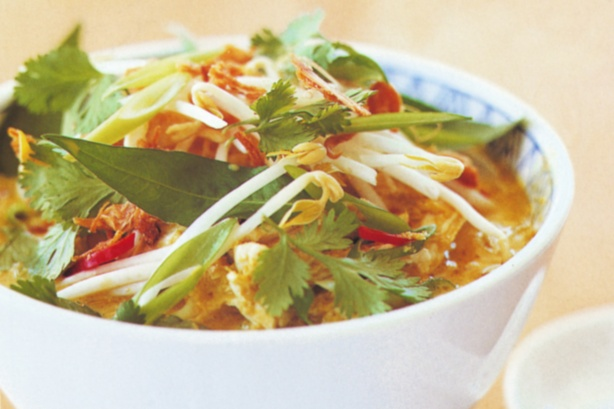
\includegraphics[scale=0.34]{./img/laksa.jpg}
		\end{textblock*}
	\item 500ml (2 cups) coconut milk
	\item 300g pkt dried rice noodles
	\item 2 single chicken breasts, steamed, sliced
	\item 1 pkt bean sprouts, straggly ends trimmed
	\item 4 spring onions, diagonally sliced
	\item 1/2 cup Vietnamese mint leaves
	\item 1/2 cup coriander leaves
	\item Fried eschallots, to serve*
\end{ingredients-list}
Laksa paste
\begin{ingredients-list}
	\item 4 large dried chillies, soaked in hot water
	\item 3 eschallots, preferably Asian (red), peeled, chopped
	\item 2 garlic cloves
	\item 3cm piece fresh ginger
	\item 2 small red chillies, seeded, chopped
	\item 4 stems lemongrass (white part only), sliced
	\item 8 macadamia nuts
	\item 1 teaspoon shrimp paste
	\item 2 teaspoons ground turmeric
	\item 2 teaspoons ground coriander
	\item 1 teaspoon palm or brown sugar
	\item 3 tablespoons peanut oil
\end{ingredients-list}

\section*{Directions}
\begin{enumerate}
	\item  To make the laksa paste, drain the chillies and place in a food processor with the eschallots, garlic, ginger, red chillies, lemongrass, nuts, shrimp paste, turmeric, coriander, sugar and 			peanut oil.  Whiz in the processor until everything is finely chopped and forms a paste. This paste can be kept in a glass jar in the fridge until needed.
	\item Heat the peanut oil in a wok over medium heat. Add the spice paste and stir-fry for about 5-6 minutes until fragrant.
	\item Add the chicken stock and coconut milk, and stir to combine. Bring to the boil, then decrease heat to medium-low and simmer for 5 minutes, stirring occasionally.
	\item Meanwhile, soak the dried rice noodles in a large bowl of boiling water for about 5 minutes until soft. Drain. Divide the noodles among serving bowls and place chicken on top.
		Ladle over the hot soup.
	\item Garnish with the bean sprouts, spring onions, Vietnamese mint leaves, coriander and fried eschallots.
\end{enumerate}
 

%%End recipe

%%End Chapter
%%Chapter - Split into separate file if too large
\chapter{Vegetarian Main Dishes}
%%Start recipe
\newrecipe{Sweet Potato and Spinach Pasta Rotolo}{http://www.jamieoliver.com/recipes/vegetables-recipes/squash-spinach-pasta-rotolo}
\section*{Ingredients}
\begin{ingredients-list}
	\item 1 butternut squash (roughly 1.2kg) (Substitute Sweet Potato)
	\item 1 red onion
	\item olive oil
	\item 1 teaspoon dried thyme
	\item 500 g frozen spinach
	\item 1 whole nutmeg, for grating
	\item 4 cloves of garlic
	\item 1 x 700 ml jar of passata
	\item 6 large fresh free-range pasta sheets (roughly 15cm x 20cm each)
	\item 50 g feta cheese
	\item20 g Parmesan cheese
\end{ingredients-list}

\section*{Directions}
\begin{enumerate}
	\item Preheat the oven to 180ºC/350ºF/gas 4. Cook the squash whole on a roasting tray for around 1 hour 30 minutes, then remove from the oven. Meanwhile, peel and roughly chop the onion, put it into a medium pan on a medium-low heat with a lug of oil, the thyme and a pinch of salt and pepper, and cook for 10 minutes, stirring occasionally. Stir in the frozen spinach, cover with a lid and allow to slowly cook for another 15 minutes, or until the liquid has evaporated, then remove from the heat. Cut the squash in half, discard the seeds and skin, then mash up with a fork. Keeping them separate, season both the squash and spinach to perfection with salt, pepper and a grating of nutmeg.  If substituting sweet potato rub the sweet potato all over with oil and place on a baking tray in the oven.  Bake for around 45 minutes to 1 hour depending on the size of the sweet potato. Skewer with a toothpick to check them but the skins should be loosened and slightly blackened when cooked.
	\item Peel and finely slice the garlic, then put it into a shallow 28cm casserole pan on a medium heat with a splash of oil and fry for a couple of minutes, or until lightly golden. Pour in the passata, then add a splash of water to the empty jar, swirl it around and pour it into the pan. Bring to the boil, simmer for just 3 minutes, then season to perfection.
	\item On a clean work surface, lay out the pasta sheets facing lengthways away from you. Working quickly so your pasta doesn't dry out, brush them with water, then evenly divide and spread the squash over the sheets. Sprinkle over the cooked spinach and crumble over the feta. Roll up the sheets and cut each one into 4 chunks, then place side by side in the tomato sauce. Finely grate over the Parmesan, then pick the sage leaves (if using), toss in a little oil and scatter over the top. Bake for 35 to 40 minutes at the bottom of the oven until golden and crisp. Delicious served with a fresh green salad.
\end{enumerate}

%%End recipe

%%End Chapter
%%Chapter - Split into separate file if too large
\chapter{Salads}

%%Start recipe
\newrecipe{Roast Tomato, Wild Rocket and Macadamia Salad}{http://www.taste.com.au/recipes/6758/roast+tomato+wild+rocket+macadamia+salad}

%\begin{figure}[h!]
%	\centering
%	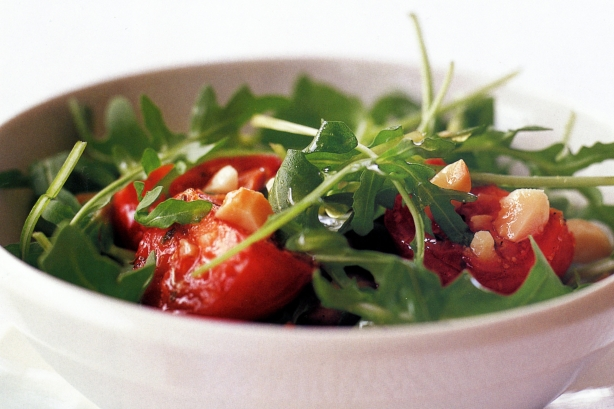
\includegraphics[scale=0.4]{./img/tomatorocketmacadamia.jpg}
%\end{figure}

\bigskip
\section*{Ingredients}

\begin{ingredients-list}
	\item 3 small vine-ripened tomatoes
		\begin{textblock*}{8cm}(8.5cm,-1.2cm) % {block width} (coords)
			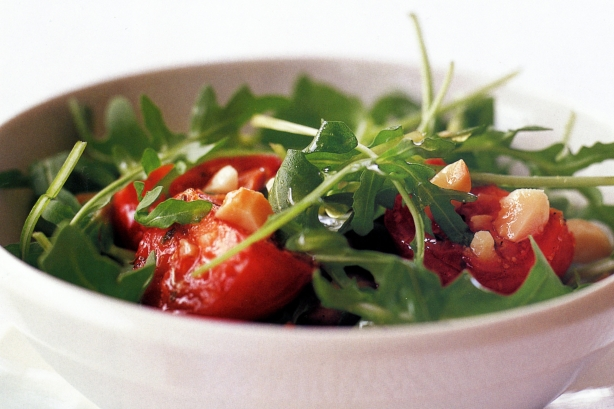
\includegraphics[scale=0.35]{./img/tomatorocketmacadamia.jpg}
		\end{textblock*}
	\item Sea Salt
	\item 300g wild rocket leaves
	\item 100g macadamia nuts, roasted, chopped
	\item 1 tsp. sugar
	\item 50ml olive oil
	\item 50ml macadamia nut oil*
	\item 40ml (2 tbsp.) white wine vinegar
	\item 1 tsp. Dijon mustard
	\item 2 tsp. Australian honey
\end{ingredients-list}

\section*{Directions}
\begin{enumerate}
	\item Cut tomatoes into quarters; add sugar, salt and pepper. Heat a non-stick pan on high heat and fry tomatoes cut-side down until slightly charred. Set aside to cool.
	\item Place the rocket, tomato and macadamias in a serving bowl.
	\item  Place remaining ingredients in a bowl and whisk to combine. Toss the dressing through the salad and serve.
\end{enumerate}
%%End recipe

%%Start recipe
\newrecipe{Fattoush\\(Middle Eastern bread salad)}{http://www.taste.com.au/recipes/6769/fattoush+middle+eastern+bread+salad}

%\begin{figure}[h!]
%	\centering
%	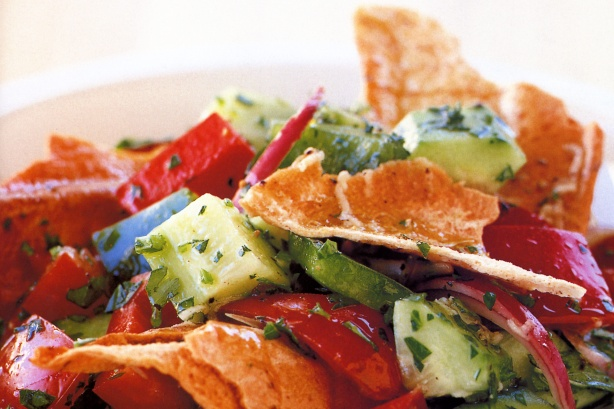
\includegraphics[scale=0.2]{./img/fattoush.jpg}
%\end{figure}
\bigskip
\section*{Ingredients}
\begin{ingredients-list}
	\item 3 small pita breads, halved
		\begin{textblock*}{8cm}(8.5cm,-1.2cm) % {block width} (coords)
			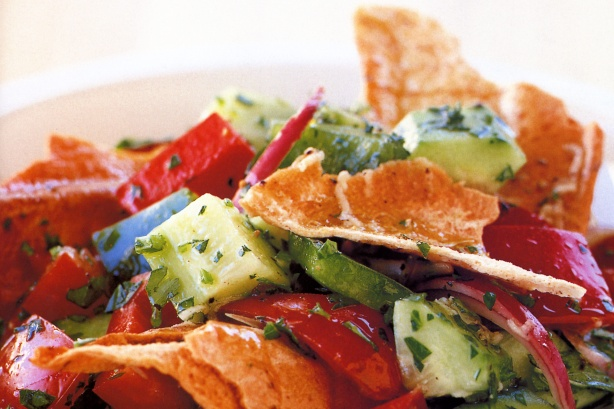
\includegraphics[scale=0.35]{./img/fattoush.jpg}
		\end{textblock*}
	\item 120ml (6 tbsp.) olive oil
	\item 2 garlic cloves, crushed
	\item 1 lemon, juiced
	\item 2 tbsp. chopped flat-leaf parsley
	\item 2 tbsp. chopped coriander leaves
	\item 2 tbsp. chopped, fresh mint leaves
	\item 1 red onion, sliced
	\item 5 tomatoes, seeded, cut into 1-2cm dice
	\item 1 telegraph cucumber, peeled, seeded,  diced into 1-2cm cubes
	\item 2 small green capsicums, seeded, diced into 1-2cm cubes
\end{ingredients-list}

\section*{Directions}
\begin{enumerate}
	\item Preheat oven to 190°C.
	\item Brush bread pieces with 2 tablespoons of the oil. Place on a baking tray and bake for 10-15 minutes until crisp and golden.
		Transfer to a plate lined with paper towel to drain and cool.
	\item Combine the garlic, lemon juice, remaining olive oil and herbs in a large bowl and season with salt and pepper.
		Add the onion, tomato, cucumber and capsicum and toss to combine.
		Just before serving, break the bread into rough pieces, add to the salad and toss well. Serve with grilled meat or fish.
\end{enumerate}
%%End Recipe

%%Start Recipe
\newrecipe{Tuna Pasta Salad}{}


\section*{Ingredients}
\begin{ingredients-list}
	\item 500g spiral pasta
	\item 1 tin (400g) of tuna
	\item 6 Sundried tomatoes cut into small strips
	\item 1 handful (20) kalamata Olives, sliced
	\item 2 Baby cos lettuce
	\item Grated parmesan cheese
	\item 50 g pine nuts
	\item 6 eggs.
	\item Anchovy Dressing from \hyperlink{salad_nicoise}{Salad nicoise recipe} on page \pageref{salad_nicoise}.
\end{ingredients-list}

\section*{Directions}
\begin{enumerate}
	\item Hard boil the eggs and leave to cool (in a sink of cold water)
	\item Toast the pine nuts in a dry frypan and set aside to cool.
	\item Cook pasta according to directions, and cool under running water.
	\item Drain the pasta well and place in large bowl with a little oil or some of the salad dressing.
		Toss lightly to prevent the pasta from sticking together.
	\item Add the chopped olives, sundried tomato strips and the remainder of the dressing and mix well.
	\item Peel the eggs and half or quarter them as desired
	\item Line bowls with the baby cos lettuce leaves and spoon in the pasta salad mixture.
	\item Garnish with eggs, pinenuts and parmesan cheese.
\end{enumerate}

%%End Recipe

%%End Chapter
%%Chapter - Split into separate file if too large
\chapter{Dips and Extras}
%% Start recipe
\newrecipe{Tomato Tapenade}{http://www.taste.com.au/recipes/10128/sun+dried+tomato+tapenade}

\section*{Ingredients}
\begin{ingredients-list}
	\item 110g (1 cup) drained sun-dried tomatoes
	\item 2 garlic cloves, peeled
	\item \sfrac{1}{2} cup firmly packed fresh basil leaves, washed, dried well
	\item 3 anchovy fillets, drained
	\item 3\sfrac{1}{2} tbs extra virgin olive oil
	\item 1\sfrac{1}{2} tsp Worcestershire sauce 
\end{ingredients-list}

\section*{Directions}
\begin{enumerate}
\item Combine sun-dried tomatoes, garlic cloves, basil leaves and anchovy fillets in the bowl of a food processor and process until roughly chopped.
\item Add 3 tbs of the extra virgin olive oil and Worcestershire sauce and process until smooth and well combined.
\item Spoon mixture into hot sterilized jars, cover surface of tapenade with the remaining extra virgin olive oil and seal immediately. Store in the fridge for up to 3 months.
\end{enumerate}
%%End Recipe

%%Begin recipe
\newrecipe{Hummus}{http://www.taste.com.au/recipes/5103/hummus}
%\begin{figure}[h!]
%\centering
%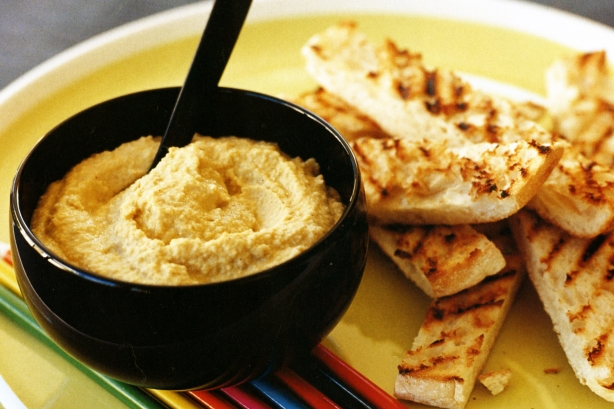
\includegraphics[scale=0.5]{img/hummus.jpg}
%\end{figure}
\bigskip
\section*{Ingredients}
\begin{ingredients-list}
	\item 600g canned chickpeas, drained, rinsed
		\begin{textblock*}{8cm}(8.5cm,-1.2cm) % {block width} (coords)
			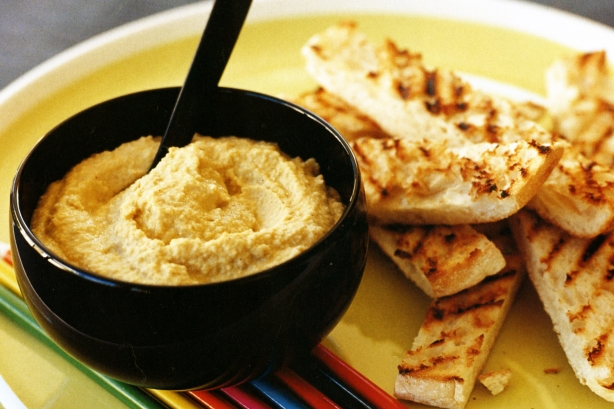
\includegraphics[scale=0.35]{./img/hummus.jpg}
		\end{textblock*}
	\item 3 garlic cloves, crushed
	\item 100ml olive oil
	\item 2 tbs tahini paste*
	\item 1 tsp ground cumin
	\item Juice of 1 lemon
	\item Toasted Turkish bread, to serve
\end{ingredients-list}

\section*{Directions}
\begin{enumerate}
	\item Place the chickpeas, garlic, olive oil, tahini paste, cumin and lemon juice in a food processor and process until combined.
		Add 1/4 cup (60ml) of water and process again until quite smooth.
	\item Place hummus in a bowl and serve with toasted Turkish bread.
\end{enumerate}
%%End recipe

%%Begin recipe
\newrecipe{Tomato Kasundi}{http://www.taste.com.au/recipes/6482/tomato+kasundi}
\label{tomato_kasundi}
\hypertarget{tomato_kasundi}{}%target for hyperlink from recipes using this recipe.
\section*{Ingredients}
\begin{ingredients-list}
	\item 60ml sunflower oil
	\item 1 tablespoon black mustard seeds
	\item 1 tablespoon turmeric
	\item 2 tablespoons cumin
	\item 2 teaspoons chilli powder
	\item \sfrac{1}{4} cup peeled, grated fresh ginger
	\item 4 crushed garlic cloves
	\item 1 seeded, finely chopped green chilli
	\item 30ml of malt vinegar
	\item 2x 400g cans diced tomatoes
	\item \sfrac{1}{3} cup brown sugar
	\item 1 teaspoon salt
	\item 130ml malt vinegar
\end{ingredients-list}

\section*{Directions}
\begin{enumerate}
	\item Heat 60ml sunflower oil in a large saucepan until hot.
		Add 1 tablespoon black mustard seeds,1 tablespoon turmeric, 2 tablespoons cumin and 2 teaspoons chilli powder.
		Cook, stirring, for 5 minutes to release the flavours.
	\item Add \sfrac{1}{4} cup peeled, grated fresh ginger, 4 crushed garlic cloves, 1 seeded, finely chopped green chilli and 30ml of malt vinegar and cook for 5 minutes.
	\item Add two 400g cans diced tomatoes, \sfrac{1}{3} cup brown sugar, 1 teaspoon salt and 130ml malt vinegar and simmer for 1-1\sfrac{1}{2} hours.
	\item The kasundi is ready when the oil comes to the top.
\end{enumerate}
%%End recipe

%%Begin recipe
\newrecipe{Caramelised Onion}{http://www.jilldupleix.com/recipes/rec052.php}
\label{caramelised_onion}
\hypertarget{caramelised_onion}{}%target for hyperlink from recipes using this recipe.

\section*{Ingredients}
\begin{ingredients-list}
\item 1 kg red (or brown) onions, peeled
\item 1 tsp. sea salt
\item \sfrac{1}{2} tsp. freshly ground black pepper
\item 2 bay leaves
\item 2 rosemary sprigs
\item 100 ml olive oil
\item 150 g soft brown sugar
\item 100 ml dry white wine
\item 75 ml red wine vinegar (Use balsamic vinegar instead)
\end{ingredients-list}

\section*{Directions}
\begin{enumerate}
\item Cut the onions in half and slice finely ( a boring task, but think of all the pleasure ahead).
	In a heavy fry pan, toss the onion in the olive oil. Cook over gentle heat until the onions start to colour.
	Add the salt, pepper, bay leaves and rosemary sprigs, cover and cook over gentle heat for 20 minutes until soft and wilted.
\item Remove the lid and add the sugar, wine and vinegar.
	Bring to the boil, stirring, then reduce the heat and cook, uncovered, for a further 20 to 30 minutes until the liquid has been absorbed by the onions, and they are soft and sticky.
	You'll need to stir fairly constantly towards the end of cooking time to avoid scorching.
\item Pick out the bay leaves and rosemary and discard. Spoon the relish into a clean, dry, sterilised jar, leave to cool, then seal tightly. Will keep in the fridge for 2 weeks.
\end{enumerate}
%%End Recipe

%%Chapter - Split into separate file if too large
\chapter{Desserts}

%%Start recipe
\newrecipe{Ricotta Custards with Macerated Strawberries}{}

%% \begin{figure}[h!]
%% \centering
%% \includegraphics[scale=0.75]{./img/image.jpg}
%% \end{figure}

\section*{Ingredients}
\begin{ingredients-list}
	\item 300 g fresh ricotta
	\item \sfrac{1}{2} cup (125ml) thickened cream
	\item 1 egg, plus 2 extra yolks
	\item \sfrac{1}{3} cup (4 tbs) honey
	\item 2 tbs roughly chopped almonds
\end{ingredients-list}
Macerated strawberries:
\begin{ingredients-list}
	\item 250g strawberries, hulled, halved if Large
	\item 1 tbs caster sugar
	\item \sfrac{1}{4} tsp finely grated orange zest
	\item 1 tbs balsamic vinegar
\end{ingredients-list}

\section*{Directions}
\begin{enumerate}
	\item Preheat the oven to 150\textcelsius.
	\item  For the macerated strawberries, place in a bowl and sprinkle with sugar
	\item Combine the orange zest and balsamic vinegar. Pour over the strawberries and toss to coat. Set aside.
	\item Firmly press ricotta through a coarse sieve into a bowl using a spatula or the back of a spoon.
		Scrape the underside of the sieve frequently. Gently fold in the cream and set aside.
	\item Place egg, egg yolks and honey in a bowl and whisk until honey is incorporated and mixtureis light and fluffy.
			Fold the egg mixture gently into the ricotta mixture.
	\item Place four \sfrac{1}{2}-cup (125ml) ramekins or ovenproof ceramic cups in a baking dish.
			Fill each ramekin with the ricotta mixture and top with the almonds.
			Fill the baking dish with enough boiling water to come halfway up the sides of the ramekins, then carefully place the baking dish in the oven.
			Bake for about 45 minutes or until the mixture is just set. Cool slightly then chill custards for 1 hour or until ready to serve.
	\item Serve the chilled ricotta custards with the macerated strawberries.
\end{enumerate}

%%End recipe


%%Start Recipe
\newrecipe{Sticky Date Pudding with Butterscotch Sauce and Almond Praline}{}

\section*{Ingredients}
\begin{ingredients-list}
	\item 180g dates, pitted and roughly chopped
	\item 1\sfrac{1}{4} cups (310ml) water
	\item \sfrac{1}{2} tsp bicarbonate of soda
	\item \sfrac{3}{4} cup (165g) firmly packed brown sugar
	\item 60g butter, softened chopped
	\item 2eggs
	\item 1 cup (150g) self-raising flour
\end{ingredients-list}
Almond praline
\begin{ingredients-list}
	\item \sfrac{1}{2} cup (110g) caster sugar
	\item \sfrac{1}{4} cup (35g) slivered almonds Butterscotch sauce
	\item 50g butter
	\item 1 cup (220g) brown sugar
	\item 1 cup (250ml) cream
	\item 1 tsp vanilla extract
\end{ingredients-list}

\section*{Directions}
\begin{enumerate}
	\item Preheat oven to 180 \textcelsius\ (160 \textcelsius\            fan·forced). Lightly grease eight (\sfrac{1}{2} cup capacity) metal dariole moulds.
	\item Place dates and water in a saucepan and bring to the boil over a high heat. Remove from the heat.
		Add bicarbonate of soda, stir until dates start to break down, set aside to cool, stirring occasionally.
	\item Beat butter and sugar in a bowl using a hand beater, gradually add eggs one at a time, beat until light and fluffy.
	\item Add date mixture, stir to combine. Carefully fold through sifted flour, divide mixture evenly between the eight moulds, until \sfrac{2}{3} full.
	\item Place moulds in a baking tray, carefully pour water in tray until it comes up \sfrac{1}{3} of the side of the moulds.
		Bake in oven for 40 minutes or until golden and skewer comes out clean.
	\item Meanwhile, for the almond praline, combine sugar and 2 tablespoons water in a saucepan over medium heat and cook caramel without stirring,
		swirling pan, until deep golden. Scatter almonds onto a baking paper·lined oven tray, pour over caramel and cool until set. Break praline into pieces.
	\item For the butterscotch sauce, combine butter, sugar, cream and vanilla in small saucepan over low heat until butter melts and sugar dissolves.
		Bring sauce to the boil, reduce heat and cook for 5·6 minutes or until sauce thickens slightly.
	\item To serve, invert the hot pudding onto a serving plate, top with butterscotch sauce and shards of praline.
\end{enumerate}
%%End Recipe

%%Start recipe
\newrecipe{Baked Strawberry Cheesecake}{http://www.kraftrecipes.com/recipes/philadelphia-classic-cheesecake-52544.aspx}

\section*{Ingredients}
\begin{ingredients-list}
	\item 1\sfrac{1}{2} cups scallywag/golliwog biscuit Crumbs
	\item 3 Tbsp. sugar
	\item \sfrac{1}{3} cup butter or margarine, melted
	\item 4 packs (250g each) PHILADELPHIA Cream Cheese/or Woolworths Homebrand, softened
	\item 1 cup sugar
	\item 1 tsp. vanilla
	\item 4eggs
\end{ingredients-list}

Stawberry Topping
\begin{ingredients-list}
	\item 2 punnets (250g each) of strawberries
	\item 1 tablespoon cornstarch
	\item 2-3 tablespoon water
\end{ingredients-list}

\section*{Directions}
\begin{enumerate}
	\item Pre-heat oven to 160 \textcelsius
	\item MIX biscuit crumbs, 3 tbsp. sugar and butter; press onto bottom of 23cm springform pan.
	\item BEAT cream cheese, 1 cup sugar and vanilla with mixer until well blended.
		Add eggs, 1 at a time, mixing on low speed after each just until blended. Pour over crust.
	\item BAKE 55 min. or until centre is almost set.
	\item Cool in the oven with the door open to avoid splitting.
	\item Loosen cake from rim of pan. Refrigerate 4 hours.
\end{enumerate}
	Strawberry Topping
\begin{enumerate}
	\item Cut the strawberries into smaller pieces (Reserve 1⁄4 - 1⁄2 for decorating)and place into a saucepan on the stovetop.
		Bring to a boil, stirring continuously for about 10 minutes. Add a small amount of water to start if needed.
	\item Add 1 cup of sugar to the mixture and stir until the sugar has melted.
	\item Mix the cornstarch with 2-3 tablespoons of water or until runny.
		Add the cornstarch to the strawberries, stirring continuously as the mixture boils for another 5 minutes.
		Remove from the stovetop.
	\item Allow the strawberry sauce to cool (place into an ice bath for faster cooling) and then blend	it in a blender until smooth.
\end{enumerate}

%%Start recipe
\newrecipe{Pear and Almond Upside Down Cake}{http://www.taste.com.au/recipes/4905/pear+almond+upside+down+cake}

\bigskip
\section*{Ingredients}

\begin{ingredients-list}
	\item 180g brown sugar
	\item 270g unsalted butter, softened
		\begin{textblock*}{8cm}(7.5cm,-1.3cm) % {block width} (coords)
			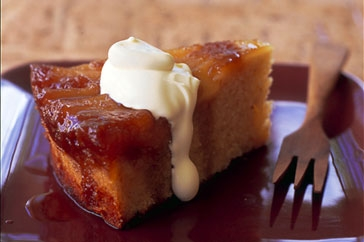
\includegraphics[scale=0.65]{./img/pear_almond.jpg}
		\end{textblock*}
	\item 300g caster sugar
	\item 3 eggs
	\item 1 \sfrac{2}{3} cups (250g) plain flour
	\item 1 \sfrac{1}{2} tsp baking powder
	\item 1 tsp ground cinnamon
	\item \sfrac{1}{2} tsp ground nutmeg
	\item 80g almond meal
	\item 1 cup (250ml) buttermilk
	\item 4 ripe pears (such as beurre bosc), peeled, cored, cut into 2cm-thick slices
	\item Thick cream, to serve 
\end{ingredients-list}

\section*{Directions}
\begin{enumerate}
	\item Preheat oven to 180°C (not fan-forced).
	\item Grease and line base of a 26cm cake pan with baking paper. Sprinkle brown sugar over base.
			Melt 100g butter and pour over brown sugar. Top with overlapping pear slices.
			Place remaining butter and caster sugar in bowl of electric mixer, beat for 5 minutes until light and fluffy.
	\item Add eggs one at a time, beating well after each addition. Sift together flour, baking powder and spices, fold into egg mixture with almond meal.
	\item Stir in buttermilk, then mix to form a smooth batter. Carefully spread over pears.
	\item Place pan on a baking tray, cook for 1 hour and 20 minutes.
	\item Cover loosely with foil if cake begins to brown too quickly. Remove and cool for 30 minutes. Run a knife around sides of pan and carefully invert onto a plate.
	\item Serve with thick cream.
\end{enumerate}
%%End recipe

%%Start recipe
\newrecipe{Blueberry Boy Bait}{http://smittenkitchen.com/blog/2009/07/blueberry-boy-bait/}

\bigskip
\section*{Ingredients}

\begin{ingredients-list}
	\item 2 cups plus 1 teaspoon all-purpose flour
	\item 1 tablespoon baking powder
		\begin{textblock*}{8cm}(8.6cm,-1.3cm) % {block width} (coords)
			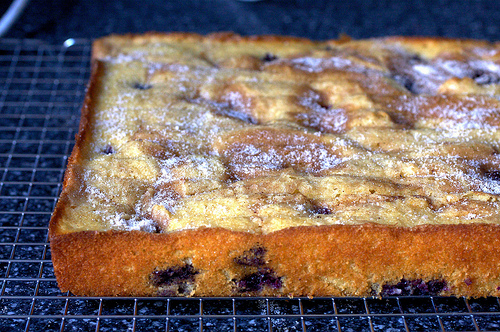
\includegraphics[scale=0.43]{./img/blueberry-boy-bait.jpg}
		\end{textblock*}
	\item 1 teaspoon table salt
	\item 250g unsalted butter (2 sticks), softened
	\item \sfrac{3}{4} cup packed light brown sugar
	\item \sfrac{1}{2} cup granulated sugar
	\item 3 large eggs
	\item 1 cup whole milk
\item \sfrac{1}{2} cup blueberries, fresh or frozen
\end{ingredients-list}

Topping
\begin{ingredients-list}
	\item \sfrac{1}{2} cup blueberries, fresh or frozen (do not defrost)
	\item \sfrac{1}{4} cup granulated sugar
	\item \sfrac{1}/{2} teaspoon ground cinnamon
\end{ingredients-list}

\section*{Directions}
\begin{enumerate}
	\item Preheat oven to 180 \textcelsius\ (170 \textcelsius\  fan-forced).
	\item Grease and 13 x 9 inch baking pan
	\item Whisk two cups flour, baking powder, and salt together in medium bowl.
		With electric mixer, beat butter and sugars on medium-high speed until fluffy, about two minutes. 
	\item Add eggs, one at a time, beating until just incorporated and scraping down bowl.
	\item Reduce speed to medium and beat in one-third of flour mixture until incorporated; beat in half of milk.
	\item Beat in half of remaining flour mixture, then remaining milk, and finally remaining flour mixture.
	\item Toss blueberries with remaining one teaspoon flour. Using rubber spatula, gently fold in blueberries.
		Spread batter into prepared pan.
	\item Scatter blueberries over top of batter.
	\item Stir together sugar and cinnamon and sprinkle over batter.
	\item Bake 45 to 50 minutes or until a toothpick inserted into centre of cake comes out clean.
	\item Cool in pan for 20 minutes then turn out and place on a serving platter.
\end{enumerate}
%%End recipe

%%Start recipe
\newrecipe{Raspberry \& Orange Upside-Down Cake}{http://www.taste.com.au/recipes/22766/raspberry+orange+upside+down+cake}

\bigskip
\section*{Ingredients}

\begin{ingredients-list}
	\item Melted butter, to grease
		\begin{textblock*}{8cm}(8.0cm,-0.8cm) % {block width} (coords)
			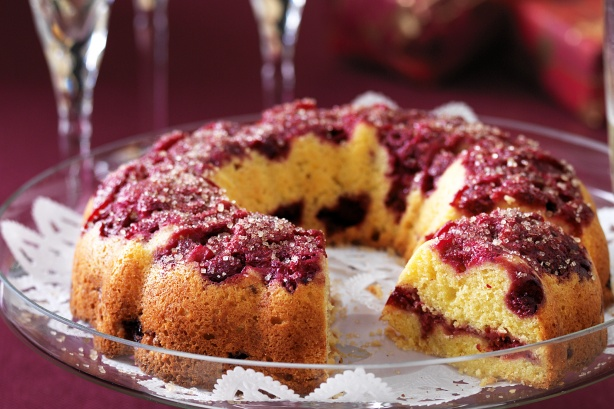
\includegraphics[scale=0.38]{./img/raspberry_orange.jpg}
		\end{textblock*}
	\item 175g butter, chopped, room temp.
	\item 155g (\sfrac{3}{4} cup) caster sugar
	\item 2 tsp finely grated orange rind
	\item 3 eggs
	\item 150g (1 cup) self-raising flour, sifted
	\item 75g (\sfrac{1}{2} cup) plain flour, sifted
	\item 100g almond meal
	\item 80ml (\sfrac{1}{3} cup) fresh orange juice
	\item 300g frozen raspberries
	\item 3 tsp demerara sugar
	\item Double or whipped cream, to serve 
\end{ingredients-list}

\section*{Directions}
\begin{enumerate}
	\item Preheat oven to 180 \textcelsius . Brush a 24cm (top measurement) fluted non-stick ring pan with melted butter to grease.
		Line the base with non-stick baking paper.
	\item Use an electric beater to beat the butter, caster sugar and orange rind in a large bowl until pale and creamy.
		Add the eggs, 1 at a time, beating well after each addition. Fold in the combined flour, almond meal and orange juice.
	\item Arrange half the raspberries in the base of the prepared pan. Top with half the cake mixture. Repeat with remaining raspberries and mixture.
		Tap on the benchtop to settle. Smooth the surface. Bake for 50-55 minutes or until a skewer inserted into the centre comes out clean.
		Set aside for 10 minutes to cool.
	\item Run a flat-bladed knife carefully around the inside edge of the pan. Turn the cake onto a cake stand or serving platter.
	\item Sprinkle with demerara sugar. Slice and serve with cream.

\end{enumerate}
%%End recipe


%%Start recipe
\newrecipe{Lemon Syrup Cake}{}

\bigskip
\section*{Ingredients}

\begin{ingredients-list}
	\item 125g butter,softened.
	\item 1\sfrac{1}{2} cup caster sugar
	\item 1 large lemon, rind finely grated, juiced
	\item 2 eggs
	\item 1\sfrac{1}{2} cup  self-raising flour, sifted
	\item \sfrac{1}{2} cup milk
\end{ingredients-list}

\section*{Directions}
\begin{enumerate}
	\item Preheat oven to 180 \textcelsius . Grease and line a 6 cm deep, 19 x10 cm base loaf pan.
	\item Use an electric beater to beat the butter, 1 cup of caster sugar and lemon rind in a large bowl until pale and creamy.
		Add the eggs, 1 at a time, beating well after each addition.
	\item Add half the flour and half the milk and stir gently to combine. Fold in the remaining flour and milk.
	\item Spoon mixture into loaf pan and bake for 45-50 minutes.
	\item Combine remaining sugar and \sfrac{1}{3} cup of lemon juice and bring to the boil.
	\item Pour over hot loaf while still in pan.  Stand in pan until cooled.

\end{enumerate}
%%End recipe


%%Start recipe
\newrecipe{Chai-spiced cakes with Earl Grey tea syrup}{http://www.taste.com.au/recipes/22380/chai+spiced+cakes+with+earl+grey+tea+syrup}

\bigskip
\section*{Ingredients}

\begin{ingredients-list}
	\item 125g butter,softened.
		\begin{textblock*}{8cm}(8.6cm,-0.8cm) % {block width} (coords)
			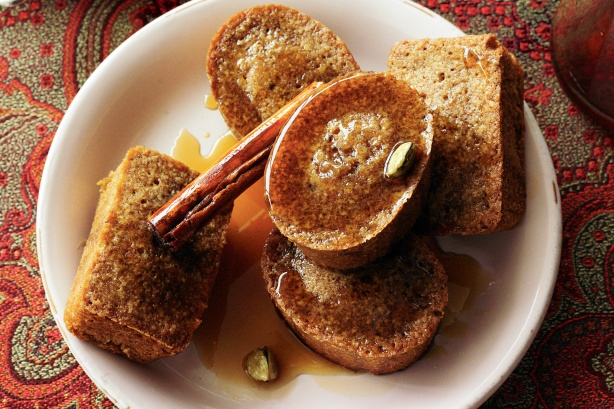
\includegraphics[scale=0.35]{./img/chai-spiced_cakes.jpg}
		\end{textblock*}
	\item 1 cup (200g) brown sugar
	\item 3 eggs
	\item sfrac{1}{2} cup (75g) plain flour
	\item sfrac{1}{4} cup (40g) self-raising flour
	\item sfrac{1}{2} cup (45g) desiccated coconut
	\item sfrac{1}{4} cup (60g) natural yoghurt
	\item 1 teaspoon ground cinnamon
	\item 1 teaspoon ground ginger
	\item \sfrac{1}{2} teaspoon ground fennel
	\item \sfrac{1}{2} teaspoon ground cardamom
	\item \sfrac{1}{2} teaspoon ground cloves
	\item Pinch ground white pepper
	\item 4 Earl Grey tea bags
	\item 1 cinnamon stick
	\item 2 cardamom pods, bruised
	\item 1 cup (250ml) boiling water
	\item \sfrac{1}{2} cup (100g) caster sugar 
\end{ingredients-list}

\section*{Directions}
\begin{enumerate}
	\item Preheat oven to 160 \textcelsius . Grease twelve 1/2-cup (125ml) capacity loaf or friand pans.
	\item Use an electric mixer to beat the butter and sugar in a medium bowl until pale and creamy.
	\item Add the eggs, one at a time, beating well between each addition until just combined.
	\item Add the flours, coconut, yoghurt, cinnamon, ginger, fennel, cardamom, cloves and pepper and stir to combine.
	\item Spoon into the prepared pans and smooth the surface.
	\item Bake in preheated oven for 20-25 minutes or until a skewer inserted in the centres comes out clean.
		Remove from oven and turn onto a wire rack to cool completely.
	\item Meanwhile, place the tea bags, cinnamon stick and cardamom pods in a medium saucepan and pour over the boiling water.
		Set aside for 5 minutes to infuse. Remove and discard the tea bags. Add the sugar and place over low heat.
		Cook, stirring, for 2 minutes or until sugar dissolves. Increase heat to high and bring to the boil.
		Cook for 5 minutes or until syrup thickens slightly. Pour over the warm cakes to serve
\end{enumerate}
%%End recipe

%%End Chapter
%%Chapter - Split into separate file if too large
\chapter{Side Dishes and Extras}

%%Start recipe
\newrecipe{Spiced Sweet Potato Mash}{}

%% \begin{figure}[h!]
%% \centering
%% \includegraphics[scale=0.75]{./img/image.jpg}
%% \end{figure}

\section*{Ingredients}
\begin{ingredients-list}
	\item 2 Sweet Potatoes, approximately same size and thickness
	\item 1 tsp. Cumin seeds
	\item 1 tsp. Caraway seeds
	\item Juice of 1 lemon
\end{ingredients-list}

\section*{Directions}
\begin{enumerate}
	\item Preheat oven to 180 C and line an oven tray with baking paper.
	\item Rub oil liberally over the skin of the sweet potatoes and bake in the oven for 40-60 minutes
		depending on thickness of the sweet potatoes.
	 Remove from the oven and allow to cool for 15-20 minutes.
	\item Dry roast the seeds in a small frypan and grind finely in a mortar and pestle
	\item Make a shallow cut lengthways and peel the skin from the sweet potato.
	\item Place the sweet potato in a bowl and mash coarsely with a fork
	\item  Add the ground spices and mix. Add lemon juice to taste.
\end{enumerate}
Can be served immediately at room temperature, or refrigerated and reheated later.


%%End recipe

%%Start Recipe
\newrecipe{Coconut Rice}{http://www.food.com/recipe/coconut-rice-126690}

\section*{Ingredients}
\begin{ingredients-list}
	\item 1 cup basmati rice
	\item 1 tablespoon olive oil
	\item \sfrac{1}{8} teaspoon salt
	\item 1 pinch saffron (about 5-6 threads)
	\item 1 cup chicken broth
	\item \sfrac{3}{4} cup coconut milk
\end{ingredients-list}

\section*{Directions}
\begin{enumerate}
	\item In a pot that has a tight-fitting lid, over high heat, add the rice, olive oil, salt, and saffron.
		Stirring with a wooden spoon, heat for 2-3 minutes until a few rice grains begin to brown on the edges.
		OPTIONAL: You may want to add a few ounces of shredded coconut at this stage.
	\item Being careful to avoid flare-ups and spill-overs, add the chicken broth and coconut milk to the hot pan. It will sizzle and bubble vigorously!
	\item  Stir to loosen any rice on the bottom or sides of the pot and reduce the heat to low. Put on the lid and cook for 13 minutes.
	\item  When 13 minutes are up, turn off the heat and let the covered rice sit for 5 minutes.
	\item Remove the lid and fluff with a fork before serving with any Asian, Polynesian, or Indian dish.
\end{enumerate}
%%End recipe

%%Start Recipe
\newrecipe{Espinacas con Garbanzos (Spinach \& Chickpeas)}{http://smittenkitchen.com/blog/2010/03/spinach-and-chickpeas/}

\section*{Ingredients}
\begin{ingredients-list}
	\item 2 420g cans of chickpeas, drained and rinsed
	\item 6 tablespoon olive oil
	\item 450g spinach, washed
	\item A hefty 1-inch slice from a country loaf or about 2 slices from sandwich loaf bread (2.5 ounces or 75 grams), crusts removed and cut inset small cubes
	\item \sfrac{1}{2} cup (4 ounces) tomato sauce
	\item 3 garlic cloves, thinly sliced
	\item 1/2 teaspoon ground cumin
	\item Pinch of red pepper flakes
	\item 1 \sfrac{1}{2} tablespoons red wine vinegar
	\item \sfrac{1}{2} teaspoon smoked paprika**
	\item Salt and freshly ground black pepper
	\item Lemon juice, to taste
\end{ingredients-list}

\section*{Directions}
\begin{enumerate}
	\item Place a large saucepan over medium heat and add half the olive oil. When it is hot, add the spinach with a pinch of salt (in batches, if necessary) and stir well.
		Remove when the leaves are just tender, drain in a colander and set aside.
	\item Heat 2 more tablespoons olive oil in a frying pan over medium heat. Fry the bread for about 5 minutes or until golden brown all over,
		 then the remaining tablespoon of oil and the garlic, cumin and pepper. Cook for 1 minute more or until the garlic is nutty brown.
	\item Transfer to a food processor, blender or mortar and pestle along with the vinegar, and mash to a paste. 
		Return the mixture to the pan and add the drained chickpeas and tomato sauce. 
		Stir until the chickpeas have absorbed the flavors and are hot. Season with salt and pepper.
\end{enumerate}
If the consistency is a little thick, add some water. Add the spinach and cook until it is hot. Check for seasoning and serve with paprika on top, or on fried bread toasts (as the Spanish do).
%%End recipe

%%Start recipe
\newrecipe{Spicy Potatoes with Pappadums}{http://www.taste.com.au/recipes/6471/spicy+potatoes+with+pappadums}

%\begin{figure}[h!]
%	\centering
%	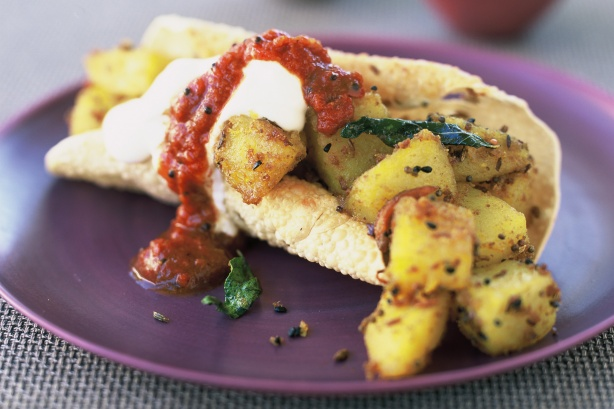
\includegraphics[scale=0.3]{./img/spicypotatoes.jpg}
%\end{figure}

\bigskip
\section*{Ingredients}
\begin{ingredients-list}
	\item 750g potatoes, peeled, cubed
		\begin{textblock*}{8cm}(6.7cm,-1.2cm) % {block width} (coords)
			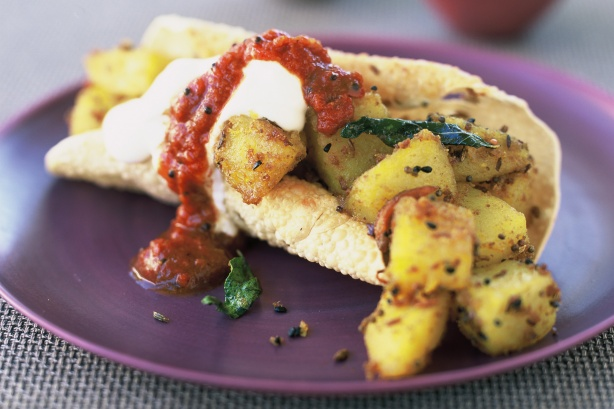
\includegraphics[scale=0.42]{./img/spicypotatoes.jpg}
		\end{textblock*}
	\item 3 tbs ghee (see Notes)
	\item \sfrac{1}{2} tsp turmeric
	\item 2 tbs panch phora 
	\item 1 tbs ground cumin
	\item 6 fresh curry leaves
	\item 1 garlic clove, crushed
	\item 1 tbs grated fresh ginger
	\item 6 large pappadums
	\item 60ml (\sfrac{1}{4} cup) lemon juice
	\item \sfrac{1}{4} cup chopped fresh coriander
	\item Tomato kasundi (see \hyperlink{tomato_kasundi}{related recipe} on page \pageref{tomato_kasundi} ) and yoghurt, if desired, to serve
\end{ingredients-list}

\section*{Directions}
\begin{enumerate}
	\item Place the potatoes in a saucepan of salted water and bring to the boil (alternatively steam them). Cook until just tender. Drain and set aside.
	\item Heat a tablespoon of the ghee in a medium frying pan.
		Add the dry spices, curry leaves, garlic and ginger and cook over medium heat for 1 minute, stirring until the flavours are released.
		Transfer to a bowl and set aside. Add 1 tablespoon of ghee to the pan; when it has melted, add potatoes (in 2 batches if necessary) and cook until golden.
		Return spice mixture to pan and cook for a further minute. Cover and set aside.
	\item Heat remaining ghee in a small frying pan over high heat.
		Carefully place 1 pappadum in the hot oil (press with tongs to help hold the shape) and fry for 2-3 seconds each side until fully expanded.
		Use tongs to transfer to paper towel to drain. Repeat with remaining pappadums.
	\item Add the lemon juice and coriander to the potatoes and reheat gently over low heat for 1-2 minutes.
	\item Place a pappadum on a serving plate, top with some spicy potatoes and the tomato kasundi. Add a dollop of yoghurt.
\end{enumerate}
%%End Recipe

%%Start recipe
\newrecipe{Super Easy Flatbreads}{http://www.jamieoliver.com/recipes/bread-recipes/easy-flatbreads}

\bigskip
\section*{Ingredients}
\begin{ingredients-list}
	\item 350g self-raising flour, plus extra for dusting
		\begin{textblock*}{8cm}(9.7cm,-2.2cm) % {block width} (coords)
			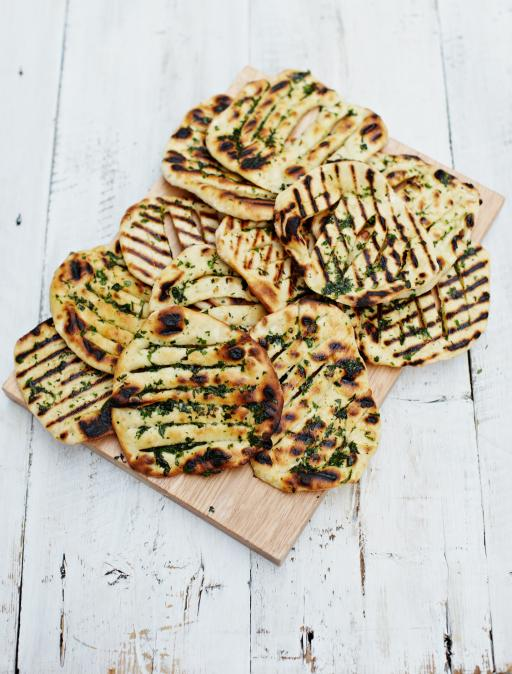
\includegraphics[scale=0.24]{./img/flatbread.jpg}
		\end{textblock*}
	\item sea salt
	\item 1 tsp baking powder
	\item 350g natural yoghurt
\end{ingredients-list}

\section*{Directions}
\begin{enumerate}
	\item Add all the flatbread ingredients to a mixing bowl and mix together with a spoon, then use clean hands to pat and bring everything together.
	\item Dust a clean work surface with flour, then tip out the dough.
	\item Knead for a minute or so to bring it all together (this isn't a traditional bread recipe, so you don't need to knead it for long – just enough time to bring everything together). 
	\item Dust a clean work surface and rolling pin with flour, then divide the dough in half, then divide each half into 6 equal-sized pieces (roughly the size of a golf ball).
	\item With your hands, pat and flatten the dough, then use a rolling pin to roll each piece into 12cm rounds, roughly 2mm to 3mm thick.
	\item Use a knife to cut 6 lines into the centre of each round, leaving about 3cm at each end.
	\item Place the griddle pan on a high heat, then once hot, cook each one for 1 to 2 minutes on each side, or until bar-marked and puffed up, turning with tongs.
	\item Brush the flatbreads all over with herby garlic butter as they come off the griddle, then pile onto a serving board so everyone can dig in and help themselves.
\end{enumerate}
Note that these work just as well without the baking powder or the cutlines in the centre.
%%End Recipe


%%End Chapter
%%Chapter - Split into separate file if too large
\chapter{Sauces and Dressings}

%%Start recipe
%% \newrecipe{Recipe name}{recipe url}

%% \begin{figure}[h!]
%% \centering
%% \includegraphics[scale=0.75]{./img/image.jpg}
%% \end{figure}

%%\section*{Ingredients}
%%\begin{ingredients-list}
%%	\item ingredient1
%%	\item ingredient2
%%\end{ingredients-list}

%% \section*{Directions}
%% \begin{enumerate}
%%	\item direction1
%%	\item direction2 etc
%%\end{enumerate}
%%End recipe

%%Start recipe
\newrecipe{Quick Satay Sauce}{}

\section*{Ingredients}
\begin{ingredients-list}
	\item 250 ml (9 fl oz/l cup) pineapple juice
	\item 250 g (9 oz/l cup) peanut butter
	\item \sfrac{1}{2} teaspoon garlic powder
	\item \sfrac{1}{2} teaspoon onion powder
	\item 2 tablespoons sweet chilli sauce
	\item 60 ml (2 fl oz/ \sfrac{1}{4} cup) soy sauce
\end{ingredients-list}

\section*{Directions}
\begin{enumerate}
	\item Combine the pineapple juice, peanut butter, garlic powder, onion powder, sweet chilli sauce and soy sauce in a small saucepan.
	\item Stir over medium heat until the mixture is smooth and heated through.
	\item Add a little water for a thinner sauce, if preferred.
	\item Reheat in a saucepan over medium heat before serving.
\end{enumerate}
%%End Recipe


%%Start Recipe
\newrecipe{Jamie Olivers Satay Sauce/Marinade}{}

\section*{Ingredients}
\begin{ingredients-list}
	\item Bunch of coriander root and stem (save the leaves)
	\item 1 large red chilli, de-seeded
	\item 1 clove of garlic
	\item 2 cm piece of fresh ginger
	\item Zest of 2 limes, juice of 1 lime
	\item 1-3 tbsp Soy sauce (add to taste for saltines)
	\item 3 tbsp. Crunchy peanut butter
	\item Water as needed to thin sauce
\end{ingredients-list}
\section*{Directions}
\begin{enumerate}
	\item Combine ingredients in a blender until you have a paste. Use the second lime’s juice to adjust acidity and add soy sauce for saltiness.
	\item Add water a little at a time to achieve spooning consistency.
\end{enumerate}
%%End Recipe

%%Start Recipe
\newrecipe{Salad Nicoise Anchovy Dressing}{}
\label{salad_nicoise}
\hypertarget{salad_nicoise}{}

\section*{Ingredients}
\begin{ingredients-list}
	\item 20 ml/4 tsp. Dijon mustard
	\item 50 g anchovy fillets
	\item 1 clove garlic crushed
	\item 60 ml/3 tbsp white wine vinegar
	\item Olive oil
\end{ingredients-list}
\section*{Directions}
\begin{enumerate}
	\item Place all ingredients in a blender with a cutting blade and process to combine.
	\item While the blender is still running add the olive oil in a thin steady stream until the dressing is	thick and creamy.
\end{enumerate}
%%End Recipe

%%End Chapter



%%The end
\end{document}